% \VignetteIndexEntry{The Jaatha HowTo}
% \VignetteDepends{jaatha}
% \VignettePackage{jaatha}

\documentclass[a4paper]{article}

\usepackage[utf8]{inputenc}
\usepackage[T1]{fontenc}
\usepackage{textcomp}

\usepackage{natbib}
\usepackage{graphics}
\usepackage{amsmath}
\usepackage{indentfirst}
\usepackage{hyperref}


\hypersetup{
	pdftitle={The Jaatha HowTo 1.9.12},
	pdfauthor={Lisha Mathew, Paul R. Staab and Dirk Metzler},
	colorlinks=true,
	linkcolor=black,          % color of internal links
	citecolor=black,        % color of links to bibliography
	filecolor=black,      % color of file links
	urlcolor=blue           % color of external links
}

\usepackage{Sweave}
\begin{document}


\title{The Jaatha HowTo}
\author{Lisha Mathew, Paul R. Staab and Dirk Metzler}
\date{Version 1.9.12}
\maketitle

\section{Introduction}
\noindent
Jaatha is a fast composite likelihood method to estimate model parameters of the
evolutionary history of (at the moment) two related species or populations.
To do so, it uses SNP data from multiple individuals from both species and -- optionally but
highly recommended -- one or more outgroup sequences.
This HowTo describes the method and gives an example of using its implementation
as an \verb@R@ package \verb@jaatha@.

The package itself can be obtained from CRAN
using
\begin{Schunk}
\begin{Sinput}
> install.packages('jaatha')
\end{Sinput}
\end{Schunk}
or downloaded from
\url{http://evol.bio.lmu.de/_statgen/software/jaatha}. Jaatha runs on all
operating systems supported by \verb@R@ -- namely Windows, OS X (Mac) and Linux
-- with one minor restriction: On Windows the parallelization is currently not
working.

A more detailed description of the algorithm can be found in
\cite{naduvilezhath_jaatha:_2011}. 
Further information about the
\verb@R@ functions used in this document can be obtained by calling 
\verb@help()@ with the functions name as argument.

Please cite the above paper when using Jaatha in a publication.


\section{A demographic model}
\noindent
Before we can apply Jaatha to estimate parameters, we first need to create a model
of the evolutionary history of the two species. Jaatha cannot account for the
effects of selection, hence we assume a neutral evolution. It can estimate the 
effects that either ``demographic'' events -- like an expansion of the
size of one population or migration between the two populations -- or molecular events --
like mutation or recombination -- have on the genome of the populations. To
emphasize that we can not include selection, we refer to a scenario of the
evolution of the two species under such events as a ``demographic model''.

For now, assume that we know that our two species are closely related; hence they must 
have separated at a certain time in the past. There may still be gene flow
ongoing between them 
to which we will refer to as migration from one population into the other. 
Hence, we could propose the simple demographic model described in Figure~\ref{fig:dm}.

\begin{figure}
\begin{center}
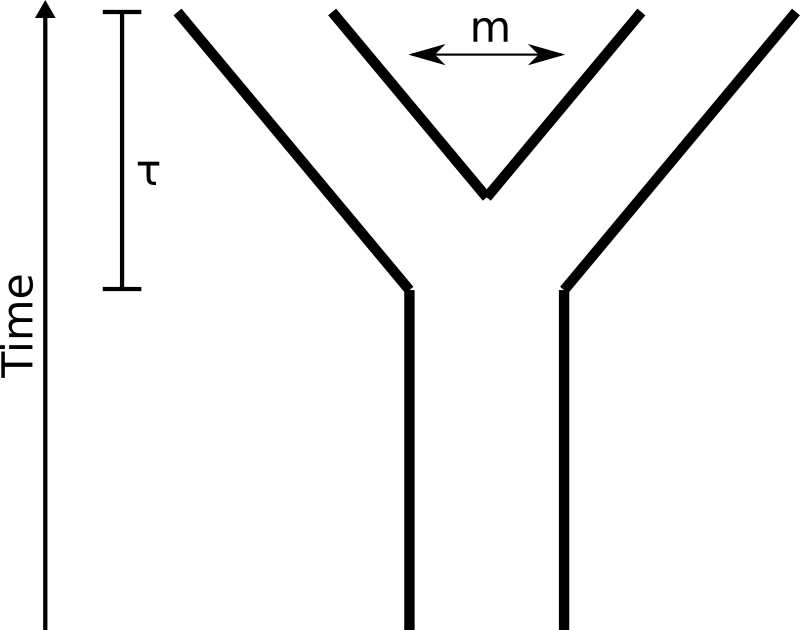
\includegraphics[width=60mm]{img/dm.png}
\end{center}
\caption{
A simple demographic model: The ancestral population splits into two populations $\tau$ time 
units ago, and afterwards individuals migrated from one population to the other with a 
migration rate $M$. Mutations are occurring with rate $\theta$ and recombination with a 
known rate $\rho$.}
\label{fig:dm}
\end{figure}

To specify that model in \verb@R@, we first need to load \verb@jaatha@.
\begin{Schunk}
\begin{Sinput}
> library(jaatha)
\end{Sinput}
\end{Schunk}
We can now create an 'empty' demographic model \verb@dm@ using the\\ 
\verb@dm.createDemographicModel()@ function:

\begin{Schunk}
\begin{Sinput}
> dm <- dm.createDemographicModel(sample.sizes=c(25,24), 
+                                 loci.num=70,
+                                 seq.length=1000)
\end{Sinput}
\end{Schunk}

The parameter \verb@sample.sizes@ here corresponds to the number of individuals we have
sampled from the first population and second population respectively. The 
second argument \verb@loci.num@ states that we are using data from $70$ loci
while \verb@seq.length@ gives the (average) length of each loci\footnote{This 
is only used when a finite sites model is assumed or if intra-locus recombination is included.}.

We can now successively add the other assumptions of our model:
\begin{Schunk}
\begin{Sinput}
> dm <- dm.addSpeciationEvent(dm, .1, 5, new.time.point.name='tau')
> dm <- dm.addSymmetricMigration(dm, .01, 5, new.par.name='M')
> dm <- dm.addMutation(dm, 1, 20, new.par.name='theta')
> dm <- dm.addRecombination(dm, fixed=20)
\end{Sinput}
\end{Schunk}
The first parameter is the demographic model to which we want to add
an assumption/feature. The two following numbers represent the range for the
coresponding parameter. 
The lower border has to be strictly greater the zero, as we are using a logarithmic transformation
of the parameter space. The parameters are scaled as in the popular simulation program
\verb@ms@ \citep{hudson_generating_2002} that we use for simulations:
\begin{itemize}
\item The parameter for the \emph{speciation} event is the split time $\tau$, which
	states how many generations ago the split of the population has occurred.
	As usual in population genetics, it is measured in units of $4N_1$ 
	generations ago, where $N_1$ is the (diploid) effective population size of 
	the first population.
\item The parameter for the (symmetric) \emph{migration} is the scaled migration rate $M$, 
	which is given by $M=4N_1m$, where $m$ is the fraction of individuals of each 
	population which are replaced by immigrants from the other population each
	generation.
\item The \emph{mutation} parameter $\theta$ is $4N_1$ times the neutral mutation
	rate per locus.
\item Finally, the \emph{recombination} parameter $\rho$ is $4N_1$ times
	the probability of recombination between the ends of the locus per generation.
\end{itemize}

\noindent
%Finally we can check your model using
%<<Checking the model>>=
%dm
%@

Keep in mind that a `good' model -- which is one that approximates the real demographic
history but is also as simple as possible -- is crucial for obtaining meaningful
estimates in the end. Jaatha will always try to find the parameters that make the
model fit best to your data. If the model does not fit to the data at all,
Jaatha will still return estimates, but they will not be meaningful.

\section{Theoretical Background}
\noindent
It is important to understand the key concepts behind Jaatha before we can apply it. Like many
estimation methods that rely on simulations, Jaatha tries to find the parameters that best fits
\footnote{for Jaatha, the 'best' parameter combination is the one with the highest
composite likelihood} to your data by simulating artificial data for many different parameter
combinations. It uses a learning algorithm to determine how the different parameter
values influence the simulated data and uses that knowledge to find the best parameter combination for 
your data. 

You can imagine Jaatha as a method that runs through the parameter space -- the space
of all possible parameter combinations, in our example a cube with borders from $0.1$ to $5$, 
$0.01$ to $5$ and $1$ to $20$ -- simulating in a small part of the parameter space
around the current position (we call this area a \emph{block}). It then searches the new maximum
of the current blocks and moves to it, builds a new block around it and so on. The search finally 
stops when the likelihood cannot be improved anymore or a maximal number of steps has been reached.

To compare the simulated data to the real one, Jaatha uses \emph{summary statistics} of the data.
As default, it calculates the Joint Site Frequency Spectrum (JSFS) of the data and further summarizes
it by evaluating different sums over the JSFS. Please refer to \cite{naduvilezhath_jaatha:_2011} for a detailed
description.


\section{Importing Your Data}
\noindent
To run Jaatha, you need to calculate the JSFS of your data. To do so, you can
use the function \verb@calculateJsfs()@. This function accepts data imported
with the \verb@read.dna()@ function from the package \emph{ape}. It assumes that you provide
a joined, aligned data set with multiple samples from two populations and -- optional 
but highly recommended -- one or more outgroup sequences. Additionally, you must
provide the numbers of the sequences in the dataset that belong to population
one, population two, and the outgroup, respectively.

Please consult the documentation of \emph{ape} in order to get more information
about \verb@read.dna()@. For example, the import of the data could look like this:  

\begin{Schunk}
\begin{Sinput}
> library(ape)
> # The path to the data
> sample.file <- system.file('example_fasta_files/sample.fasta', 
+                            package='jaatha')
> # Reading the data
> sample.data <- read.dna(sample.file, format='fasta', 
+                         as.character=TRUE)
> # Calculating the JSFS
> sample.jsfs <- calculateJsfs(sample.data, 
+                              pop1.rows=3:7, 
+                              pop2.rows=8:12,
+                              outgroup.row=1:2)
> sample.jsfs
\end{Sinput}
\begin{Soutput}
     [,1] [,2] [,3] [,4] [,5] [,6]
[1,]    1    0    0    0    0    0
[2,]    1    1    1    0    0    0
[3,]    2    0    1    0    0    0
[4,]    1    1    0    2    0    1
[5,]    1    0    0    0    3    0
[6,]    1    0    0    0    0    0
\end{Soutput}
\end{Schunk}

\vspace{1em}
\noindent
For the purpose of this HowTo, we will use a simulated JSFS, for which we 
know the real parameters:

\begin{Schunk}
\begin{Sinput}
> # Real parameters: M = 1, tau = 1 and theta = 10
> real.pars <- c(1,1,10) 
> # Simulate a JSFS with this parameters
> jsfs <- dm.simSumStats(dm, real.pars)
> # Print the upper left part of the JSFS
> jsfs[1:10, 1:10]
\end{Sinput}
\begin{Soutput}
      [,1] [,2] [,3] [,4] [,5] [,6] [,7] [,8] [,9] [,10]
 [1,]    0  760  345  219  141   91   80   57   69    29
 [2,]  659   39   27   32   26   17   12    6   17    10
 [3,]  333   20   19   14    9    5   14    7    9     5
 [4,]  177   14   14   21    9    6   10    6    1     9
 [5,]  173   17   21   13    7    7   10    8   10     6
 [6,]  109   19   21   13    2    6    6    4    4     4
 [7,]   71   21   12    3    6    7    7    5    5     2
 [8,]   69   13    7    9    4    8    6    3    3     0
 [9,]   56   20    3    6    6    3    0    3    3     1
[10,]   44   17    5   11    5    4    1    1    0     0
\end{Soutput}
\end{Schunk}

\section{Running Jaatha}

\noindent
Jaatha is divided into two parts. First we find good starting
positions by simulating very coarsely across the entire parameter space. We call
this part \emph{initial search}. Afterwards a more thorough \emph{refined search}
is performed starting from the best positions of the first step. Before starting
the search, we need to set some options like our demographic model, the summary 
statistics of the real data, and a seed to ensure repoducibilty:

\begin{Schunk}
\begin{Sinput}
> jaatha <- Jaatha.initialize(dm, jsfs=jsfs, seed=12345)
\end{Sinput}
\end{Schunk}


\noindent
For more options refer to \verb@?Jaatha.initialize@ or the Jaatha manual.

\subsection{The Initial Search}

\noindent
For the initial search, we divide the parameter space into equally-sized blocks by dividing 
each of the $n$ parameters ranges into \verb@nBlocksPerPar@ intervals such that we obtain 
$($\verb@nBlocksPerPar@$)^n$ blocks. Within each block we simulate \verb@nSim@ data sets with 
-- on a logarithmic scale -- uniformly drawn parameter values within each block. To ensure 
a better sampling of the edges, we simulate in addition data sets for all corner points of 
each parameter block.

For these data sets we then fit the GLMs and estimate the parameter combination with the
maximal score\footnote{In this phase, Jaatha uses a score instead of the
likelihood for computational reasons. The likelihood is proportional to $\exp(\text{score})$. 
The higher the score, the higher the likelihood.}. 
Each of the blocks provides a single best parameter combination.

In R, the initial search is performed with the command

% Don't run a complete jaatha search; would take tooo long

\begin{Schunk}
\begin{Sinput}
> start.points <- Jaatha.initialSearch(jaatha, nSim=100, nBlocksPerPar=3)
\end{Sinput}
\begin{Soutput}
externalTheta set to TRUE for initial search. 
*** Starting position is being determined *** 
Creating 9 initial blocks ...  
*** Block 1  (lowerB: 0.1 0.01  upperB: 0.368 0.079 ) 
Best parameters:  0.137 0.079 0.761 | Score: 48292.1 

*** Block 2  (lowerB: 0.1 0.079  upperB: 0.368 0.63 ) 
Best parameters:  0.221 0.63 0.739 | Score: 48517.92 

*** Block 3  (lowerB: 0.1 0.63  upperB: 0.368 5 ) 
Best parameters:  0.336 0.8 0.705 | Score: 48594.04 

*** Block 4  (lowerB: 0.368 0.01  upperB: 1.357 0.079 ) 
Best parameters:  0.368 0.079 0.691 | Score: 47261.71 

*** Block 5  (lowerB: 0.368 0.079  upperB: 1.357 0.63 ) 
Best parameters:  0.407 0.63 0.684 | Score: 48656.31 

*** Block 6  (lowerB: 0.368 0.63  upperB: 1.357 5 ) 
Best parameters:  0.706 0.884 0.671 | Score: 48756.83 

*** Block 7  (lowerB: 1.357 0.01  upperB: 5 0.079 ) 
Best parameters:  1.357 0.079 0.607 | Score: 44017.74 

*** Block 8  (lowerB: 1.357 0.079  upperB: 5 0.63 ) 
Best parameters:  1.357 0.63 0.615 | Score: 48529.36 

*** Block 9  (lowerB: 1.357 0.63  upperB: 5 5 ) 
Best parameters:  1.357 0.858 0.617 | Score: 48726.59 

         score t_split_1     M theta
 [1,] 48756.83     0.706 0.884 0.671
 [2,] 48726.59     1.357 0.858 0.617
 [3,] 48656.31     0.407 0.630 0.684
 [4,] 48594.04     0.336 0.800 0.705
 [5,] 48529.36     1.357 0.630 0.615
 [6,] 48517.92     0.221 0.630 0.739
 [7,] 48292.10     0.137 0.079 0.761
 [8,] 47261.71     0.368 0.079 0.691
 [9,] 44017.74     1.357 0.079 0.607
\end{Soutput}
\end{Schunk}




\noindent
To visualise the estimates for good stating positions sorted by sorce, type:
\begin{Schunk}
\begin{Sinput}
> Jaatha.printStartPoints(jaatha, start.points)
\end{Sinput}
\begin{Soutput}
         score   tau     M  theta
 [1,] 32123.74 1.357 1.015  9.320
 [2,] 32112.91 0.858 1.092 10.464
 [3,] 32023.98 0.275 0.876 12.332
 [4,] 31983.12 0.368 0.630 11.090
 [5,] 31980.47 0.176 0.630 13.383
 [6,] 31905.78 1.357 0.630  8.869
 [7,] 31867.61 0.111 0.079 13.964
 [8,] 31024.21 0.368 0.079 10.859
 [9,] 28449.97 1.357 0.079  8.725
\end{Soutput}
\end{Schunk}
Here, there is a big reduction in the scores after the first seven blocks, and a smaller one 
after the first two. This is suggesting that we either use the first two or the
first seven 
blocks as starting positions for the refined search, depending on how much time we want to
spend. For now, we will just use the first two points.
\begin{Schunk}
\begin{Sinput}
> picked.points <- Jaatha.pickBestStartPoints(start.points, 2)
\end{Sinput}
\begin{Soutput}
There used to be 9 blocks in the list.
Keeping Block: 9  6  
\end{Soutput}
\end{Schunk}


\subsection{The Refined Search}


\noindent
Now we can conduct the more thorough refined search described above to improve the
likelihood approximations. 


\begin{Schunk}
\begin{Sinput}
> jaatha <- Jaatha.refineSearch(jaatha, picked.points, nSim=100)
\end{Sinput}
\begin{Soutput}
*** Search with starting Point in Block 1 of 2 **** 
----------------- 
Step No 1 
Number of blocks kept: 0  / Number of blocks deleted: 0 
Best parameters:  1.65 0.915 7.375 | Score: 47309.61 

----------------- 
Step No 2 
Number of blocks kept: 1  / Number of blocks deleted: 0 
Best parameters:  1.498 0.945 8.566 | Score: 47449.22 

----------------- 
Step No 3 
Number of blocks kept: 1  / Number of blocks deleted: 1 
Best parameters:  1.232 0.969 9.446 | Score: 47481.35 

----------------- 
Step No 4 
Number of blocks kept: 1  / Number of blocks deleted: 1 
Best parameters:  1.083 0.967 9.704 | Score: 47481.77 

----------------- 
Step No 5 
Number of blocks kept: 1  / Number of blocks deleted: 1 
Best parameters:  1.019 0.981 9.805 | Score: 47484.12 

----------------- 
Step No 6 
Number of blocks kept: 2  / Number of blocks deleted: 0 
Best parameters:  1.013 0.978 9.804 | Score: 47484.57 

----------------- 
Step No 7 
Number of blocks kept: 3  / Number of blocks deleted: 0 
Best parameters:  1.005 0.977 9.828 | Score: 47484.44 

----------------- 
Step No 8 
Number of blocks kept: 3  / Number of blocks deleted: 1 
Best parameters:  1.022 0.978 9.81 | Score: 47483.93 

----------------- 
Step No 9 
Number of blocks kept: 4  / Number of blocks deleted: 0 
Best parameters:  1.016 0.976 9.815 | Score: 47483.81 

----------------- 
Step No 10 
Number of blocks kept: 5  / Number of blocks deleted: 0 
Best parameters:  1.024 0.975 9.805 | Score: 47484.27 

*** Finished search *** 
Likelihood value has not change much in the last 5 steps. 
Seems we have converged. 

Calulating composite log likelihoods for best estimates: 
Parameter combination 1 of 10 ... 
Parameter combination 2 of 10 ... 
Parameter combination 3 of 10 ... 
Parameter combination 4 of 10 ... 
Parameter combination 5 of 10 ... 
Parameter combination 6 of 10 ... 
Parameter combination 7 of 10 ... 
Parameter combination 8 of 10 ... 
Parameter combination 9 of 10 ... 
Parameter combination 10 of 10 ... 
1	-89.2513	1.024472	0.9754111	9.804571	NA	
*** Search with starting Point in Block 2 of 2 **** 
----------------- 
Step No 1 
Number of blocks kept: 0  / Number of blocks deleted: 0 
Best parameters:  0.914 1.009 8.537 | Score: 47386.63 

----------------- 
Step No 2 
Number of blocks kept: 1  / Number of blocks deleted: 0 
Best parameters:  0.973 0.993 9.871 | Score: 47482.09 

----------------- 
Step No 3 
Number of blocks kept: 1  / Number of blocks deleted: 1 
Best parameters:  1.024 0.973 9.801 | Score: 47483.06 

----------------- 
Step No 4 
Number of blocks kept: 2  / Number of blocks deleted: 0 
Best parameters:  1.042 0.967 9.776 | Score: 47483.64 

----------------- 
Step No 5 
Number of blocks kept: 3  / Number of blocks deleted: 0 
Best parameters:  1.041 0.969 9.763 | Score: 47483.86 

----------------- 
Step No 6 
Number of blocks kept: 4  / Number of blocks deleted: 0 
Best parameters:  1.041 0.969 9.766 | Score: 47483.99 

----------------- 
Step No 7 
Number of blocks kept: 5  / Number of blocks deleted: 0 
Best parameters:  1.045 0.968 9.756 | Score: 47484.13 

----------------- 
Step No 8 
Number of blocks kept: 6  / Number of blocks deleted: 0 
Best parameters:  1.045 0.971 9.757 | Score: 47484.24 

*** Finished search *** 
Likelihood value has not change much in the last 5 steps. 
Seems we have converged. 

Calulating composite log likelihoods for best estimates: 
Parameter combination 1 of 10 ... 
Parameter combination 2 of 10 ... 
Parameter combination 3 of 10 ... 
Parameter combination 4 of 10 ... 
Parameter combination 5 of 10 ... 
Parameter combination 6 of 10 ... 
Parameter combination 7 of 10 ... 
Parameter combination 8 of 10 ... 
Parameter combination 9 of 10 ... 
Parameter combination 10 of 10 ... 
2	-90.03684	1.040644	0.9687806	9.762802	NA	

Best log-composite-likelihood values are: 
     log.cl block t_split_1         M    theta
1 -89.25130     1 1.0244721 0.9754111 9.804571
5 -90.03684     2 1.0406436 0.9687806 9.762802
3 -90.34609     2 1.0240919 0.9727450 9.801191
4 -90.62973     1 1.0830957 0.9674488 9.703678
2 -90.96667     2 0.9730808 0.9932475 9.871250
\end{Soutput}
\end{Schunk}



\noindent
Hence we perform two independent searches, starting in the two \verb@startPoints@ we choose before 
and according to the general options we choose during initialization, which are stored in the 
\verb@jaatha@ object. In each step, we build a block with \verb@halfBlockSize@ in each direction
(on a logarithmic scale) and perform simulations for \verb@nSim@ random parameter combinations within
this block (plus one for very corner). We use this information to estimate the composite maximum 
likelihood parameters within this block and take this value as new starting position for the next
step. 

The algorithm stops when the score has not changed more than \verb@epsilon@ for five consecutive 
steps or step \verb@nMaxStep@ is reached. To avoid getting stuck in local maxima, 
the \verb@weight@ option decreases the weight of simulations of previous blocks.

Finally the log composite likelihoods for the best ten parameter combinations are 
approximated using \verb@nFinalSim@ simulations. These are values printed at the 
end of the search. This matrix can also be accessed via

\begin{Schunk}
\begin{Sinput}
> likelihoods <- Jaatha.printLikelihoods(jaatha)
> print(likelihoods[1:3, ])
\end{Sinput}
\begin{Soutput}
     log.cl block       tau        M    theta
1 -86.12714     2 0.9739440 1.032511 10.25657
7 -86.18361     1 0.9885422 1.026013 10.31083
4 -86.73760     2 1.0280078 1.021425 10.22406
\end{Soutput}
\end{Schunk}

%\begin{figure}
%  \begin{center}
%<<<label=fig1,fig=TRUE,echo=FALSE>>=
%<<printLT>>
%@
%  \end{center}
%  \caption{Likelihoods sorted by value}
%  \label{fig:one}
%\end{figure}

\section{Parallelization}
On Linux and OS X, Jaatha can distribute the simulations on multiple CPU cores.
To use this feature, set the \verb@cores@ option during initialization. The
value of the option specifies the number of cores you want to use. As default,
Jaatha will execute 'packages' of 10 simulation on a core in a row to reduce the
overhead created by inter-process communication. This is fine for demographic
models that can be quickly simulated. However, if you have simulations that takes
multiple seconds and/or many cores available, you may want smaller packages.
This can be archived by setting \verb@sim.package.size = 1@.

The use of the \verb@cores@ option does affect the seeding system. A run without
\verb@cores@ will give different results as the identical run with the option
set at a value greater than one, even when using the same seed. However, if you
use \verb@cores@, the actual number of cores you use does not change the
results.

\bibliographystyle{plainnat}
\bibliography{jaatha}

\end{document}
